\documentclass[tikz]{standalone}

\usetikzlibrary{matrix, positioning, automata, arrows}

\begin{document}

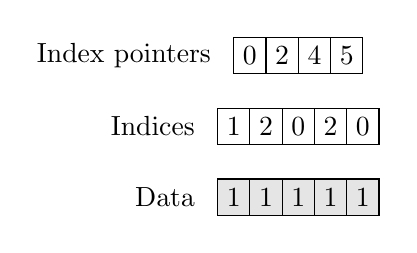
\begin{tikzpicture}[
    2d-arr/.style={matrix of nodes, row sep=-\pgflinewidth, column sep=-\pgflinewidth, nodes={draw}}
  ]

%% this array contains the increasing number of non zero elements in each row starting from zero
%% first element is always 0, then first row has two non zero elements -> 0+2, second row has 2 non zero elments -> 0+2+2 etc..
    \matrix (R) [2d-arr, nodes={draw}] {
    0 & 2 & 4 & 5 \\
  };
    \node[left=0.1 em of R] {Index pointers};

    \matrix (C) [2d-arr, below=0.5em of R, nodes={draw}] {
    1 & 2 & 0 & 2 & 0  \\
  };
  \node[left=0.1 em of C] {Indices};

    \matrix (D) [2d-arr, below=0.5em of C, nodes={draw, fill=gray!20}] {
    1 & 1 & 1 & 1 & 1  \\
  };
  \node[left=0.1em of D] {Data};

\end{tikzpicture}

\end{document}